\documentclass[a4paper,11pt]{article}
\input{/home/tof/Documents/Cozy/latex-include/preambule_doc.tex}
\input{/home/tof/Documents/Cozy/latex-include/preambule_commun.tex}
\newcommand{\showprof}{show them}  % comment this line if you don't want to see todo environment
\setlength{\fboxrule}{0.8pt}
\fancyhead[L]{\fbox{\Large{\textbf{SysExp 04}}}}
\fancyhead[C]{\textbf{TP Terminus}}
\newdate{madate}{10}{09}{2020}
%\fancyhead[R]{\displaydate{madate}} %\today
%\fancyhead[R]{Seconde - SNT}
\fancyhead[R]{Première - NSI}
%\fancyhead[R]{Terminale - NSI}
\fancyfoot[L]{\vspace{1mm}Christophe Viroulaud}
\AtEndDocument{\label{lastpage}}
\fancyfoot[C]{\textbf{Page \thepage/\pageref{lastpage}}}
\fancyfoot[R]{\includegraphics[width=2cm,align=t]{/home/tof/Documents/Cozy/latex-include/cc.png}}
\usepackage{tikz}
\usetikzlibrary{shapes.multipart}
\begin{document}
\section{Problématique}
Nous avons l'habitude d'interagir avec le système d'exploitation grâce à son interface graphique (bureau, explorateur\dots). Il reste cependant pertinent de savoir utiliser les commandes \emph{en mode console} lors de l'intervention sur un serveur à distance par exemple.
\begin{center}
    \framebox{Quelles commandes principales permettent d'interagir avec le système d'exploitation?}
\end{center}
\section{Terminus}
Pour mémoriser les commandes, il faut manipuler encore et encore. Le jeu sérieux \emph{Terminus} propose de s'entraîner à travers une petite aventure. L'objectif est de parcourir les salles (les répertoires), interagir avec les personnages ou les objets (les fichiers), réaliser des sorts (les commandes).
\begin{activite}
\begin{enumerate}
    \item Se rendre sur \url{http://luffah.xyz/bidules/Terminus/}
    \item Commencer le jeu en entrant un nom et en validant.
    \item Au fur et à mesure de l'avancement dans la partie, maintenir sur une feuille:
    \begin{itemize}
        \item un plan du jeu (voir le modèle figure \ref{modele}),
        \item un tableau des commandes et leur utilité (figure \ref{tab}).
    \end{itemize}
\end{enumerate}
\end{activite}
\begin{center}
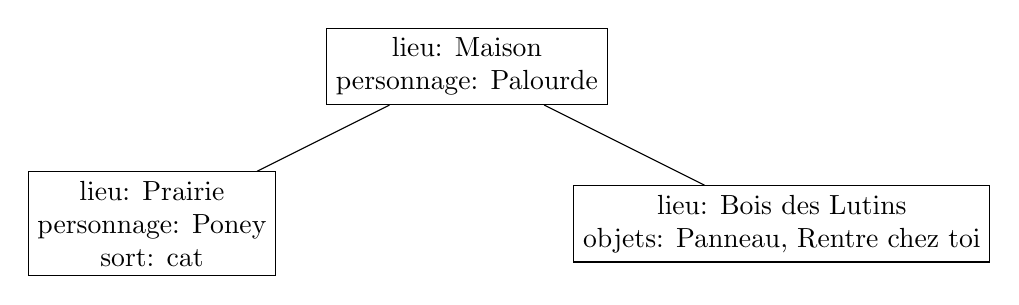
\begin{tikzpicture}[every text node part/.style={align=center}]
\node[rectangle, draw] (A) at (0,0) {lieu: Maison \\ personnage: Palourde};
\node[rectangle, draw] (B) at (-4,-2) {lieu: Prairie \\ personnage: Poney \\ sort: cat};
\node[rectangle, draw] (C) at (4,-2) {lieu: Bois des Lutins \\ objets: Panneau, Rentre chez toi};

\draw (A)--(B);
\draw (A)--(C);
\end{tikzpicture}
\captionof{figure}{Modèle de plan}
\label{modele}
\end{center}
\begin{center}
    \begin{tabular}{|*{3}{c|}}
        \hline
        commande & description & utilisation dans le jeu \\
        \hline
        cat & Examiner en détail & Interagir avec un objet\\
        \hline
    \end{tabular}
    \captionof{figure}{Exemple de tableau}
    \label{tab}
\end{center}
\end{document}